\documentclass[1p]{elsarticle_modified}
%\bibliographystyle{elsarticle-num}

%\usepackage[colorlinks]{hyperref}
%\usepackage{abbrmath_seonhwa} %\Abb, \Ascr, \Acal ,\Abf, \Afrak
\usepackage{amsfonts}
\usepackage{amssymb}
\usepackage{amsmath}
\usepackage{amsthm}
\usepackage{scalefnt}
\usepackage{amsbsy}
\usepackage{kotex}
\usepackage{caption}
\usepackage{subfig}
\usepackage{color}
\usepackage{graphicx}
\usepackage{xcolor} %% white, black, red, green, blue, cyan, magenta, yellow
\usepackage{float}
\usepackage{setspace}
\usepackage{hyperref}

\usepackage{tikz}
\usetikzlibrary{arrows}

\usepackage{multirow}
\usepackage{array} % fixed length table
\usepackage{hhline}

%%%%%%%%%%%%%%%%%%%%%
\makeatletter
\renewcommand*\env@matrix[1][\arraystretch]{%
	\edef\arraystretch{#1}%
	\hskip -\arraycolsep
	\let\@ifnextchar\new@ifnextchar
	\array{*\c@MaxMatrixCols c}}
\makeatother %https://tex.stackexchange.com/questions/14071/how-can-i-increase-the-line-spacing-in-a-matrix
%%%%%%%%%%%%%%%

\usepackage[normalem]{ulem}

\newcommand{\msout}[1]{\ifmmode\text{\sout{\ensuremath{#1}}}\else\sout{#1}\fi}
%SOURCE: \msout is \stkout macro in https://tex.stackexchange.com/questions/20609/strikeout-in-math-mode

\newcommand{\cancel}[1]{
	\ifmmode
	{\color{red}\msout{#1}}
	\else
	{\color{red}\sout{#1}}
	\fi
}

\newcommand{\add}[1]{
	{\color{blue}\uwave{#1}}
}

\newcommand{\replace}[2]{
	\ifmmode
	{\color{red}\msout{#1}}{\color{blue}\uwave{#2}}
	\else
	{\color{red}\sout{#1}}{\color{blue}\uwave{#2}}
	\fi
}

\newcommand{\Sol}{\mathcal{S}} %segment
\newcommand{\D}{D} %diagram
\newcommand{\A}{\mathcal{A}} %arc


%%%%%%%%%%%%%%%%%%%%%%%%%%%%%5 test

\def\sl{\operatorname{\textup{SL}}(2,\Cbb)}
\def\psl{\operatorname{\textup{PSL}}(2,\Cbb)}
\def\quan{\mkern 1mu \triangleright \mkern 1mu}

\theoremstyle{definition}
\newtheorem{thm}{Theorem}[section]
\newtheorem{prop}[thm]{Proposition}
\newtheorem{lem}[thm]{Lemma}
\newtheorem{ques}[thm]{Question}
\newtheorem{cor}[thm]{Corollary}
\newtheorem{defn}[thm]{Definition}
\newtheorem{exam}[thm]{Example}
\newtheorem{rmk}[thm]{Remark}
\newtheorem{alg}[thm]{Algorithm}

\newcommand{\I}{\sqrt{-1}}
\begin{document}

%\begin{frontmatter}
%
%\title{Boundary parabolic representations of knots up to 8 crossings}
%
%%% Group authors per affiliation:
%\author{Yunhi Cho} 
%\address{Department of Mathematics, University of Seoul, Seoul, Korea}
%\ead{yhcho@uos.ac.kr}
%
%
%\author{Seonhwa Kim} %\fnref{s_kim}}
%\address{Center for Geometry and Physics, Institute for Basic Science, Pohang, 37673, Korea}
%\ead{ryeona17@ibs.re.kr}
%
%\author{Hyuk Kim}
%\address{Department of Mathematical Sciences, Seoul National University, Seoul 08826, Korea}
%\ead{hyukkim@snu.ac.kr}
%
%\author{Seokbeom Yoon}
%\address{Department of Mathematical Sciences, Seoul National University, Seoul, 08826,  Korea}
%\ead{sbyoon15@snu.ac.kr}
%
%\begin{abstract}
%We find all boundary parabolic representation of knots up to 8 crossings.
%
%\end{abstract}
%\begin{keyword}
%    \MSC[2010] 57M25 
%\end{keyword}
%
%\end{frontmatter}

%\linenumbers
%\tableofcontents
%
\newcommand\colored[1]{\textcolor{white}{\rule[-0.35ex]{0.8em}{1.4ex}}\kern-0.8em\color{red} #1}%
%\newcommand\colored[1]{\textcolor{white}{ #1}\kern-2.17ex	\textcolor{white}{ #1}\kern-1.81ex	\textcolor{white}{ #1}\kern-2.15ex\color{red}#1	}

{\Large $\underline{12a_{0333}~(K12a_{0333})}$}

\setlength{\tabcolsep}{10pt}
\renewcommand{\arraystretch}{1.6}
\vspace{1cm}\begin{tabular}{m{100pt}>{\centering\arraybackslash}m{274pt}}
\multirow{5}{120pt}{
	\centering
	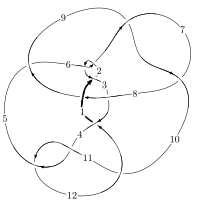
\includegraphics[width=112pt]{../../../GIT/diagram.site/Diagrams/png/1134_12a_0333.png}\\
\ \ \ A knot diagram\footnotemark}&
\allowdisplaybreaks
\textbf{Linearized knot diagam} \\
\cline{2-2}
 &
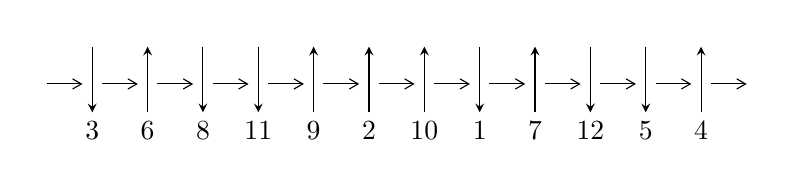
\begin{tikzpicture}[x=20pt, y=17pt]
	% nodes
	\node (C0) at (0, 0) {};
	\node (C1) at (1, 0) {};
	\node (C1U) at (1, +1) {};
	\node (C1D) at (1, -1) {3};

	\node (C2) at (2, 0) {};
	\node (C2U) at (2, +1) {};
	\node (C2D) at (2, -1) {6};

	\node (C3) at (3, 0) {};
	\node (C3U) at (3, +1) {};
	\node (C3D) at (3, -1) {8};

	\node (C4) at (4, 0) {};
	\node (C4U) at (4, +1) {};
	\node (C4D) at (4, -1) {11};

	\node (C5) at (5, 0) {};
	\node (C5U) at (5, +1) {};
	\node (C5D) at (5, -1) {9};

	\node (C6) at (6, 0) {};
	\node (C6U) at (6, +1) {};
	\node (C6D) at (6, -1) {2};

	\node (C7) at (7, 0) {};
	\node (C7U) at (7, +1) {};
	\node (C7D) at (7, -1) {10};

	\node (C8) at (8, 0) {};
	\node (C8U) at (8, +1) {};
	\node (C8D) at (8, -1) {1};

	\node (C9) at (9, 0) {};
	\node (C9U) at (9, +1) {};
	\node (C9D) at (9, -1) {7};

	\node (C10) at (10, 0) {};
	\node (C10U) at (10, +1) {};
	\node (C10D) at (10, -1) {12};

	\node (C11) at (11, 0) {};
	\node (C11U) at (11, +1) {};
	\node (C11D) at (11, -1) {5};

	\node (C12) at (12, 0) {};
	\node (C12U) at (12, +1) {};
	\node (C12D) at (12, -1) {4};
	\node (C13) at (13, 0) {};

	% arrows
	\draw[->,>={angle 60}]
	(C0) edge (C1) (C1) edge (C2) (C2) edge (C3) (C3) edge (C4) (C4) edge (C5) (C5) edge (C6) (C6) edge (C7) (C7) edge (C8) (C8) edge (C9) (C9) edge (C10) (C10) edge (C11) (C11) edge (C12) (C12) edge (C13) ;	\draw[->,>=stealth]
	(C1U) edge (C1D) (C2D) edge (C2U) (C3U) edge (C3D) (C4U) edge (C4D) (C5D) edge (C5U) (C6D) edge (C6U) (C7D) edge (C7U) (C8U) edge (C8D) (C9D) edge (C9U) (C10U) edge (C10D) (C11U) edge (C11D) (C12D) edge (C12U) ;
	\end{tikzpicture} \\
\hhline{~~} \\& 
\textbf{Solving Sequence} \\ \cline{2-2} 
 &
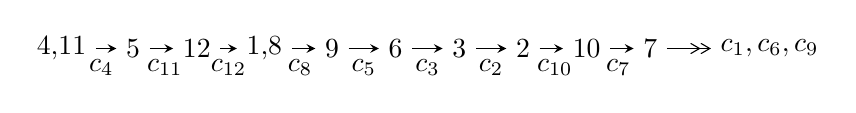
\begin{tikzpicture}[x=23pt, y=7pt]
	% node
	\node (A0) at (-1/8, 0) {4,11};
	\node (A1) at (1, 0) {5};
	\node (A2) at (2, 0) {12};
	\node (A3) at (49/16, 0) {1,8};
	\node (A4) at (33/8, 0) {9};
	\node (A5) at (41/8, 0) {6};
	\node (A6) at (49/8, 0) {3};
	\node (A7) at (57/8, 0) {2};
	\node (A8) at (65/8, 0) {10};
	\node (A9) at (73/8, 0) {7};
	\node (C1) at (1/2, -1) {$c_{4}$};
	\node (C2) at (3/2, -1) {$c_{11}$};
	\node (C3) at (5/2, -1) {$c_{12}$};
	\node (C4) at (29/8, -1) {$c_{8}$};
	\node (C5) at (37/8, -1) {$c_{5}$};
	\node (C6) at (45/8, -1) {$c_{3}$};
	\node (C7) at (53/8, -1) {$c_{2}$};
	\node (C8) at (61/8, -1) {$c_{10}$};
	\node (C9) at (69/8, -1) {$c_{7}$};
	\node (A10) at (11, 0) {$c_{1},c_{6},c_{9}$};

	% edge
	\draw[->,>=stealth]	
	(A0) edge (A1) (A1) edge (A2) (A2) edge (A3) (A3) edge (A4) (A4) edge (A5) (A5) edge (A6) (A6) edge (A7) (A7) edge (A8) (A8) edge (A9) ;
	\draw[->>,>={angle 60}]	
	(A9) edge (A10);
\end{tikzpicture} \\ 

\end{tabular} \\

\footnotetext{
The image of knot diagram is generated by the software ``\textbf{Draw programme}" developed by Andrew Bartholomew(\url{http://www.layer8.co.uk/maths/draw/index.htm\#Running-draw}), where we modified some parts for our purpose(\url{https://github.com/CATsTAILs/LinksPainter}).
}\phantom \\ \newline 
\centering \textbf{Ideals for irreducible components\footnotemark of $X_{\text{par}}$} 
 
\begin{align*}
I^u_{1}&=\langle 
1.20734\times10^{126} u^{119}+2.46333\times10^{126} u^{118}+\cdots+3.54053\times10^{125} b+4.43052\times10^{125},\\
\phantom{I^u_{1}}&\phantom{= \langle  }3.79147\times10^{125} u^{119}+1.43350\times10^{125} u^{118}+\cdots+3.54053\times10^{125} a-4.94486\times10^{125},\;u^{120}+3 u^{119}+\cdots+2 u+1\rangle \\
\\
\end{align*}
\raggedright * 1 irreducible components of $\dim_{\mathbb{C}}=0$, with total 120 representations.\\
\footnotetext{All coefficients of polynomials are rational numbers. But the coefficients are sometimes approximated in decimal forms when there is not enough margin.}
\newpage
\renewcommand{\arraystretch}{1}
\centering \section*{I. $I^u_{1}= \langle 1.21\times10^{126} u^{119}+2.46\times10^{126} u^{118}+\cdots+3.54\times10^{125} b+4.43\times10^{125},\;3.79\times10^{125} u^{119}+1.43\times10^{125} u^{118}+\cdots+3.54\times10^{125} a-4.94\times10^{125},\;u^{120}+3 u^{119}+\cdots+2 u+1 \rangle$}
\flushleft \textbf{(i) Arc colorings}\\
\begin{tabular}{m{7pt} m{180pt} m{7pt} m{180pt} }
\flushright $a_{4}=$&$\begin{pmatrix}1\\0\end{pmatrix}$ \\
\flushright $a_{11}=$&$\begin{pmatrix}0\\u\end{pmatrix}$ \\
\flushright $a_{5}=$&$\begin{pmatrix}1\\u^2\end{pmatrix}$ \\
\flushright $a_{12}=$&$\begin{pmatrix}- u\\- u^3+u\end{pmatrix}$ \\
\flushright $a_{1}=$&$\begin{pmatrix}- u^3\\- u^3+u\end{pmatrix}$ \\
\flushright $a_{8}=$&$\begin{pmatrix}-1.07088 u^{119}-0.404884 u^{118}+\cdots-1.06912 u+1.39664\\-3.41004 u^{119}-6.95753 u^{118}+\cdots-4.08476 u-1.25137\end{pmatrix}$ \\
\flushright $a_{9}=$&$\begin{pmatrix}-1.10879 u^{119}-0.667261 u^{118}+\cdots-1.24150 u+1.18917\\-3.20538 u^{119}-6.69967 u^{118}+\cdots-4.21800 u-1.27669\end{pmatrix}$ \\
\flushright $a_{6}=$&$\begin{pmatrix}-6.11682 u^{119}-9.64072 u^{118}+\cdots-0.615382 u-3.46092\\-4.22643 u^{119}-6.06316 u^{118}+\cdots+5.77722 u-1.25101\end{pmatrix}$ \\
\flushright $a_{3}=$&$\begin{pmatrix}9.55745 u^{119}+15.8859 u^{118}+\cdots+8.75147 u+4.29676\\4.22090 u^{119}+7.00859 u^{118}+\cdots+16.1434 u+8.70903\end{pmatrix}$ \\
\flushright $a_{2}=$&$\begin{pmatrix}11.4755 u^{119}+27.6957 u^{118}+\cdots+10.6546 u+7.38802\\2.78667 u^{119}+10.9141 u^{118}+\cdots+11.1166 u+3.67666\end{pmatrix}$ \\
\flushright $a_{10}=$&$\begin{pmatrix}u^3\\u^5- u^3+u\end{pmatrix}$ \\
\flushright $a_{7}=$&$\begin{pmatrix}-1.49406 u^{119}-1.43715 u^{118}+\cdots-1.45193 u+0.634651\\-4.21529 u^{119}-8.96618 u^{118}+\cdots-7.00577 u-1.78600\end{pmatrix}$\\&\end{tabular}
\flushleft \textbf{(ii) Obstruction class $= -1$}\\~\\
\flushleft \textbf{(iii) Cusp Shapes $= -1.73851 u^{119}-7.21969 u^{118}+\cdots-14.7819 u-2.34006$}\\~\\
\newpage\renewcommand{\arraystretch}{1}
\flushleft \textbf{(iv) u-Polynomials at the component}\newline \\
\begin{tabular}{m{50pt}|m{274pt}}
Crossings & \hspace{64pt}u-Polynomials at each crossing \\
\hline $$\begin{aligned}c_{1}\end{aligned}$$&$\begin{aligned}
&u^{120}+45 u^{119}+\cdots-34 u^2+1
\end{aligned}$\\
\hline $$\begin{aligned}c_{2},c_{6}\end{aligned}$$&$\begin{aligned}
&u^{120}- u^{119}+\cdots-6 u^3+1
\end{aligned}$\\
\hline $$\begin{aligned}c_{3}\end{aligned}$$&$\begin{aligned}
&u^{120}-49 u^{119}+\cdots-10414 u+557
\end{aligned}$\\
\hline $$\begin{aligned}c_{4},c_{11}\end{aligned}$$&$\begin{aligned}
&u^{120}+3 u^{119}+\cdots+2 u+1
\end{aligned}$\\
\hline $$\begin{aligned}c_{5}\end{aligned}$$&$\begin{aligned}
&u^{120}+45 u^{119}+\cdots+7856120 u+971617
\end{aligned}$\\
\hline $$\begin{aligned}c_{7},c_{9}\end{aligned}$$&$\begin{aligned}
&u^{120}+u^{119}+\cdots+28 u+1
\end{aligned}$\\
\hline $$\begin{aligned}c_{8}\end{aligned}$$&$\begin{aligned}
&u^{120}+5 u^{119}+\cdots+12 u+1
\end{aligned}$\\
\hline $$\begin{aligned}c_{10}\end{aligned}$$&$\begin{aligned}
&u^{120}+59 u^{119}+\cdots+6 u^2+1
\end{aligned}$\\
\hline $$\begin{aligned}c_{12}\end{aligned}$$&$\begin{aligned}
&u^{120}+9 u^{119}+\cdots-404318 u+65969
\end{aligned}$\\
\hline
\end{tabular}\\~\\
\newpage\renewcommand{\arraystretch}{1}
\flushleft \textbf{(v) Riley Polynomials at the component}\newline \\
\begin{tabular}{m{50pt}|m{274pt}}
Crossings & \hspace{64pt}Riley Polynomials at each crossing \\
\hline $$\begin{aligned}c_{1}\end{aligned}$$&$\begin{aligned}
&y^{120}+61 y^{119}+\cdots-68 y+1
\end{aligned}$\\
\hline $$\begin{aligned}c_{2},c_{6}\end{aligned}$$&$\begin{aligned}
&y^{120}+45 y^{119}+\cdots-34 y^2+1
\end{aligned}$\\
\hline $$\begin{aligned}c_{3}\end{aligned}$$&$\begin{aligned}
&y^{120}-603 y^{119}+\cdots-24727612 y+310249
\end{aligned}$\\
\hline $$\begin{aligned}c_{4},c_{11}\end{aligned}$$&$\begin{aligned}
&y^{120}-59 y^{119}+\cdots+6 y^2+1
\end{aligned}$\\
\hline $$\begin{aligned}c_{5}\end{aligned}$$&$\begin{aligned}
&y^{120}-639 y^{119}+\cdots-56197112480332 y+944039594689
\end{aligned}$\\
\hline $$\begin{aligned}c_{7},c_{9}\end{aligned}$$&$\begin{aligned}
&y^{120}-79 y^{119}+\cdots+108 y+1
\end{aligned}$\\
\hline $$\begin{aligned}c_{8}\end{aligned}$$&$\begin{aligned}
&y^{120}-3 y^{119}+\cdots-60 y+1
\end{aligned}$\\
\hline $$\begin{aligned}c_{10}\end{aligned}$$&$\begin{aligned}
&y^{120}+5 y^{119}+\cdots+12 y+1
\end{aligned}$\\
\hline $$\begin{aligned}c_{12}\end{aligned}$$&$\begin{aligned}
&y^{120}+49 y^{119}+\cdots-260893161688 y+4351908961
\end{aligned}$\\
\hline
\end{tabular}\\~\\
\newpage\flushleft \textbf{(vi) Complex Volumes and Cusp Shapes}
$$\begin{array}{c|c|c}  
\text{Solutions to }I^u_{1}& \I (\text{vol} + \sqrt{-1}CS) & \text{Cusp shape}\\
 \hline 
\begin{aligned}
u &= -0.979856 + 0.344337 I \\
a &= \phantom{-}1.09366 + 0.96908 I \\
b &= -0.363071 + 0.138763 I\end{aligned}
 & \phantom{-}0.62225 - 3.02138 I & \phantom{-0.000000 } 0 \\ \hline\begin{aligned}
u &= -0.979856 - 0.344337 I \\
a &= \phantom{-}1.09366 - 0.96908 I \\
b &= -0.363071 - 0.138763 I\end{aligned}
 & \phantom{-}0.62225 + 3.02138 I & \phantom{-0.000000 } 0 \\ \hline\begin{aligned}
u &= \phantom{-}0.324737 + 0.902702 I \\
a &= \phantom{-}0.276812 + 0.016151 I \\
b &= \phantom{-}0.489944 - 0.577252 I\end{aligned}
 & \phantom{-}4.18323 + 3.09968 I & \phantom{-0.000000 } 0 \\ \hline\begin{aligned}
u &= \phantom{-}0.324737 - 0.902702 I \\
a &= \phantom{-}0.276812 - 0.016151 I \\
b &= \phantom{-}0.489944 + 0.577252 I\end{aligned}
 & \phantom{-}4.18323 - 3.09968 I & \phantom{-0.000000 } 0 \\ \hline\begin{aligned}
u &= -0.171558 + 0.943685 I \\
a &= -0.193763 - 0.269957 I \\
b &= \phantom{-}0.112001 - 0.316899 I\end{aligned}
 & \phantom{-}1.92595 + 3.80713 I & \phantom{-0.000000 } 0 \\ \hline\begin{aligned}
u &= -0.171558 - 0.943685 I \\
a &= -0.193763 + 0.269957 I \\
b &= \phantom{-}0.112001 + 0.316899 I\end{aligned}
 & \phantom{-}1.92595 - 3.80713 I & \phantom{-0.000000 } 0 \\ \hline\begin{aligned}
u &= -0.761541 + 0.710272 I \\
a &= -0.529374 - 0.492267 I \\
b &= -0.672411 + 1.215670 I\end{aligned}
 & \phantom{-}6.12981 + 11.58910 I & \phantom{-0.000000 } 0 \\ \hline\begin{aligned}
u &= -0.761541 - 0.710272 I \\
a &= -0.529374 + 0.492267 I \\
b &= -0.672411 - 1.215670 I\end{aligned}
 & \phantom{-}6.12981 - 11.58910 I & \phantom{-0.000000 } 0 \\ \hline\begin{aligned}
u &= \phantom{-}0.767501 + 0.722782 I \\
a &= \phantom{-}0.575940 - 0.354501 I \\
b &= \phantom{-}0.498118 + 1.157700 I\end{aligned}
 & \phantom{-}7.84829 - 5.50381 I & \phantom{-0.000000 } 0 \\ \hline\begin{aligned}
u &= \phantom{-}0.767501 - 0.722782 I \\
a &= \phantom{-}0.575940 + 0.354501 I \\
b &= \phantom{-}0.498118 - 1.157700 I\end{aligned}
 & \phantom{-}7.84829 + 5.50381 I & \phantom{-0.000000 } 0\\
 \hline 
 \end{array}$$\newpage$$\begin{array}{c|c|c}  
\text{Solutions to }I^u_{1}& \I (\text{vol} + \sqrt{-1}CS) & \text{Cusp shape}\\
 \hline 
\begin{aligned}
u &= \phantom{-}0.976991 + 0.397527 I \\
a &= -1.28088 + 0.80343 I \\
b &= \phantom{-}0.254492 - 0.367447 I\end{aligned}
 & \phantom{-}1.34359 - 1.89187 I & \phantom{-0.000000 } 0 \\ \hline\begin{aligned}
u &= \phantom{-}0.976991 - 0.397527 I \\
a &= -1.28088 - 0.80343 I \\
b &= \phantom{-}0.254492 + 0.367447 I\end{aligned}
 & \phantom{-}1.34359 + 1.89187 I & \phantom{-0.000000 } 0 \\ \hline\begin{aligned}
u &= -0.677820 + 0.808170 I \\
a &= -0.197815 - 0.094008 I \\
b &= -0.528005 + 0.471225 I\end{aligned}
 & \phantom{-}0.18750 + 3.33247 I & \phantom{-0.000000 } 0 \\ \hline\begin{aligned}
u &= -0.677820 - 0.808170 I \\
a &= -0.197815 + 0.094008 I \\
b &= -0.528005 - 0.471225 I\end{aligned}
 & \phantom{-}0.18750 - 3.33247 I & \phantom{-0.000000 } 0 \\ \hline\begin{aligned}
u &= -1.05515\phantom{ +0.000000I} \\
a &= -1.05269\phantom{ +0.000000I} \\
b &= -0.630172\phantom{ +0.000000I}\end{aligned}
 & -1.68544\phantom{ +0.000000I} & \phantom{-0.000000 } 0 \\ \hline\begin{aligned}
u &= -0.834199 + 0.699354 I \\
a &= -0.954568 + 0.410532 I \\
b &= \phantom{-}0.467867 + 1.072280 I\end{aligned}
 & \phantom{-}5.92230 - 6.26866 I & \phantom{-0.000000 } 0 \\ \hline\begin{aligned}
u &= -0.834199 - 0.699354 I \\
a &= -0.954568 - 0.410532 I \\
b &= \phantom{-}0.467867 - 1.072280 I\end{aligned}
 & \phantom{-}5.92230 + 6.26866 I & \phantom{-0.000000 } 0 \\ \hline\begin{aligned}
u &= -0.813951 + 0.398465 I \\
a &= -0.429377 + 1.103900 I \\
b &= \phantom{-}0.160266 + 0.083993 I\end{aligned}
 & -1.81976 + 1.21553 I & \phantom{-0.000000 } 0 \\ \hline\begin{aligned}
u &= -0.813951 - 0.398465 I \\
a &= -0.429377 - 1.103900 I \\
b &= \phantom{-}0.160266 - 0.083993 I\end{aligned}
 & -1.81976 - 1.21553 I & \phantom{-0.000000 } 0 \\ \hline\begin{aligned}
u &= \phantom{-}0.831410 + 0.719173 I \\
a &= \phantom{-}0.820300 + 0.252864 I \\
b &= -0.264529 + 1.037440 I\end{aligned}
 & \phantom{-}7.66835 + 0.09297 I & \phantom{-0.000000 } 0\\
 \hline 
 \end{array}$$\newpage$$\begin{array}{c|c|c}  
\text{Solutions to }I^u_{1}& \I (\text{vol} + \sqrt{-1}CS) & \text{Cusp shape}\\
 \hline 
\begin{aligned}
u &= \phantom{-}0.831410 - 0.719173 I \\
a &= \phantom{-}0.820300 - 0.252864 I \\
b &= -0.264529 - 1.037440 I\end{aligned}
 & \phantom{-}7.66835 - 0.09297 I & \phantom{-0.000000 } 0 \\ \hline\begin{aligned}
u &= \phantom{-}0.290332 + 0.844265 I \\
a &= \phantom{-}0.412571 + 0.243861 I \\
b &= \phantom{-}0.96998 - 1.22147 I\end{aligned}
 & \phantom{-}5.15191 + 8.18955 I & \phantom{-0.000000 } 0 \\ \hline\begin{aligned}
u &= \phantom{-}0.290332 - 0.844265 I \\
a &= \phantom{-}0.412571 - 0.243861 I \\
b &= \phantom{-}0.96998 + 1.22147 I\end{aligned}
 & \phantom{-}5.15191 - 8.18955 I & \phantom{-0.000000 } 0 \\ \hline\begin{aligned}
u &= -0.316699 + 0.831772 I \\
a &= -0.260078 + 0.219002 I \\
b &= -1.115100 - 0.753088 I\end{aligned}
 & -1.89051 - 6.35992 I & \phantom{-0.000000 } 0 \\ \hline\begin{aligned}
u &= -0.316699 - 0.831772 I \\
a &= -0.260078 - 0.219002 I \\
b &= -1.115100 + 0.753088 I\end{aligned}
 & -1.89051 + 6.35992 I & \phantom{-0.000000 } 0 \\ \hline\begin{aligned}
u &= \phantom{-}1.089150 + 0.234904 I \\
a &= \phantom{-}1.80307 + 0.24588 I \\
b &= \phantom{-}1.018600 + 0.404078 I\end{aligned}
 & -4.15140 - 4.50015 I & \phantom{-0.000000 } 0 \\ \hline\begin{aligned}
u &= \phantom{-}1.089150 - 0.234904 I \\
a &= \phantom{-}1.80307 - 0.24588 I \\
b &= \phantom{-}1.018600 - 0.404078 I\end{aligned}
 & -4.15140 + 4.50015 I & \phantom{-0.000000 } 0 \\ \hline\begin{aligned}
u &= -0.286154 + 0.838179 I \\
a &= -0.415933 + 0.302299 I \\
b &= -1.12271 - 1.31896 I\end{aligned}
 & \phantom{-}3.4719 - 14.1532 I & \phantom{-0.000000 } 0 \\ \hline\begin{aligned}
u &= -0.286154 - 0.838179 I \\
a &= -0.415933 - 0.302299 I \\
b &= -1.12271 + 1.31896 I\end{aligned}
 & \phantom{-}3.4719 + 14.1532 I & \phantom{-0.000000 } 0 \\ \hline\begin{aligned}
u &= -0.698078 + 0.518282 I \\
a &= -0.00357 + 1.74069 I \\
b &= \phantom{-}0.684357 - 0.598030 I\end{aligned}
 & \phantom{-}1.02759 + 6.71407 I & \phantom{-0.000000 } 0. - 9.53783 I\\
 \hline 
 \end{array}$$\newpage$$\begin{array}{c|c|c}  
\text{Solutions to }I^u_{1}& \I (\text{vol} + \sqrt{-1}CS) & \text{Cusp shape}\\
 \hline 
\begin{aligned}
u &= -0.698078 - 0.518282 I \\
a &= -0.00357 - 1.74069 I \\
b &= \phantom{-}0.684357 + 0.598030 I\end{aligned}
 & \phantom{-}1.02759 - 6.71407 I & \phantom{-0.000000 -}0. + 9.53783 I \\ \hline\begin{aligned}
u &= \phantom{-}1.044660 + 0.435012 I \\
a &= -2.23762 + 0.53331 I \\
b &= -0.719465 - 1.126900 I\end{aligned}
 & -0.02482 - 2.22257 I & \phantom{-0.000000 } 0 \\ \hline\begin{aligned}
u &= \phantom{-}1.044660 - 0.435012 I \\
a &= -2.23762 - 0.53331 I \\
b &= -0.719465 + 1.126900 I\end{aligned}
 & -0.02482 + 2.22257 I & \phantom{-0.000000 } 0 \\ \hline\begin{aligned}
u &= \phantom{-}1.020500 + 0.498431 I \\
a &= -0.652839 + 0.488485 I \\
b &= \phantom{-}0.092070 - 1.215700 I\end{aligned}
 & \phantom{-}3.23486 - 0.38929 I & \phantom{-0.000000 } 0 \\ \hline\begin{aligned}
u &= \phantom{-}1.020500 - 0.498431 I \\
a &= -0.652839 - 0.488485 I \\
b &= \phantom{-}0.092070 + 1.215700 I\end{aligned}
 & \phantom{-}3.23486 + 0.38929 I & \phantom{-0.000000 } 0 \\ \hline\begin{aligned}
u &= -1.076580 + 0.378949 I \\
a &= \phantom{-}1.15257 + 1.55328 I \\
b &= \phantom{-}0.769790 + 0.474045 I\end{aligned}
 & -2.77897 + 1.18278 I & \phantom{-0.000000 } 0 \\ \hline\begin{aligned}
u &= -1.076580 - 0.378949 I \\
a &= \phantom{-}1.15257 - 1.55328 I \\
b &= \phantom{-}0.769790 - 0.474045 I\end{aligned}
 & -2.77897 - 1.18278 I & \phantom{-0.000000 } 0 \\ \hline\begin{aligned}
u &= -1.032920 + 0.505731 I \\
a &= \phantom{-}0.245975 + 0.413112 I \\
b &= -0.073973 - 1.102930 I\end{aligned}
 & \phantom{-}3.37682 + 5.48598 I & \phantom{-0.000000 } 0 \\ \hline\begin{aligned}
u &= -1.032920 - 0.505731 I \\
a &= \phantom{-}0.245975 - 0.413112 I \\
b &= -0.073973 + 1.102930 I\end{aligned}
 & \phantom{-}3.37682 - 5.48598 I & \phantom{-0.000000 } 0 \\ \hline\begin{aligned}
u &= -1.091040 + 0.431738 I \\
a &= \phantom{-}4.85889 + 5.71513 I \\
b &= \phantom{-}4.89829 + 0.38098 I\end{aligned}
 & -1.02292 + 5.65821 I & \phantom{-0.000000 } 0\\
 \hline 
 \end{array}$$\newpage$$\begin{array}{c|c|c}  
\text{Solutions to }I^u_{1}& \I (\text{vol} + \sqrt{-1}CS) & \text{Cusp shape}\\
 \hline 
\begin{aligned}
u &= -1.091040 - 0.431738 I \\
a &= \phantom{-}4.85889 - 5.71513 I \\
b &= \phantom{-}4.89829 - 0.38098 I\end{aligned}
 & -1.02292 - 5.65821 I & \phantom{-0.000000 } 0 \\ \hline\begin{aligned}
u &= \phantom{-}0.660166 + 0.493992 I \\
a &= -0.29803 + 1.59123 I \\
b &= -0.445578 - 0.769412 I\end{aligned}
 & \phantom{-}2.13373 - 1.83530 I & \phantom{-}5.17783 + 4.58003 I \\ \hline\begin{aligned}
u &= \phantom{-}0.660166 - 0.493992 I \\
a &= -0.29803 - 1.59123 I \\
b &= -0.445578 + 0.769412 I\end{aligned}
 & \phantom{-}2.13373 + 1.83530 I & \phantom{-}5.17783 - 4.58003 I \\ \hline\begin{aligned}
u &= -1.131570 + 0.329651 I \\
a &= \phantom{-}1.19322 + 0.96903 I \\
b &= \phantom{-}0.869209 + 0.761560 I\end{aligned}
 & -3.37533 + 0.37024 I & \phantom{-0.000000 } 0 \\ \hline\begin{aligned}
u &= -1.131570 - 0.329651 I \\
a &= \phantom{-}1.19322 - 0.96903 I \\
b &= \phantom{-}0.869209 - 0.761560 I\end{aligned}
 & -3.37533 - 0.37024 I & \phantom{-0.000000 } 0 \\ \hline\begin{aligned}
u &= -1.075110 + 0.492379 I \\
a &= -1.13838 - 1.46213 I \\
b &= -1.27344 - 0.72132 I\end{aligned}
 & \phantom{-}0.47500 + 4.53395 I & \phantom{-0.000000 } 0 \\ \hline\begin{aligned}
u &= -1.075110 - 0.492379 I \\
a &= -1.13838 + 1.46213 I \\
b &= -1.27344 + 0.72132 I\end{aligned}
 & \phantom{-}0.47500 - 4.53395 I & \phantom{-0.000000 } 0 \\ \hline\begin{aligned}
u &= \phantom{-}1.141380 + 0.312790 I \\
a &= -1.40861 + 0.91446 I \\
b &= -1.054980 + 0.838300 I\end{aligned}
 & -4.89679 + 4.65011 I & \phantom{-0.000000 } 0 \\ \hline\begin{aligned}
u &= \phantom{-}1.141380 - 0.312790 I \\
a &= -1.40861 - 0.91446 I \\
b &= -1.054980 - 0.838300 I\end{aligned}
 & -4.89679 - 4.65011 I & \phantom{-0.000000 } 0 \\ \hline\begin{aligned}
u &= \phantom{-}1.096310 + 0.460123 I \\
a &= \phantom{-}11.4019 - 26.8572 I \\
b &= \phantom{-}19.2908 - 7.8522 I\end{aligned}
 & -0.82002 - 1.64527 I & \phantom{-0.000000 } 0\\
 \hline 
 \end{array}$$\newpage$$\begin{array}{c|c|c}  
\text{Solutions to }I^u_{1}& \I (\text{vol} + \sqrt{-1}CS) & \text{Cusp shape}\\
 \hline 
\begin{aligned}
u &= \phantom{-}1.096310 - 0.460123 I \\
a &= \phantom{-}11.4019 + 26.8572 I \\
b &= \phantom{-}19.2908 + 7.8522 I\end{aligned}
 & -0.82002 + 1.64527 I & \phantom{-0.000000 } 0 \\ \hline\begin{aligned}
u &= -1.18948\phantom{ +0.000000I} \\
a &= -0.950978\phantom{ +0.000000I} \\
b &= -0.616281\phantom{ +0.000000I}\end{aligned}
 & -1.66019\phantom{ +0.000000I} & \phantom{-0.000000 } 0 \\ \hline\begin{aligned}
u &= -0.702662 + 0.388268 I \\
a &= \phantom{-}0.601372 + 0.300948 I \\
b &= -1.097330 - 0.318766 I\end{aligned}
 & \phantom{-}0.79969 - 2.86212 I & \phantom{-}1.25285 + 0.98098 I \\ \hline\begin{aligned}
u &= -0.702662 - 0.388268 I \\
a &= \phantom{-}0.601372 - 0.300948 I \\
b &= -1.097330 + 0.318766 I\end{aligned}
 & \phantom{-}0.79969 + 2.86212 I & \phantom{-}1.25285 - 0.98098 I \\ \hline\begin{aligned}
u &= -1.115540 + 0.439696 I \\
a &= -0.398178 + 1.288090 I \\
b &= \phantom{-}0.419244 + 0.947562 I\end{aligned}
 & -2.49083 + 1.59231 I & \phantom{-0.000000 } 0 \\ \hline\begin{aligned}
u &= -1.115540 - 0.439696 I \\
a &= -0.398178 - 1.288090 I \\
b &= \phantom{-}0.419244 - 0.947562 I\end{aligned}
 & -2.49083 - 1.59231 I & \phantom{-0.000000 } 0 \\ \hline\begin{aligned}
u &= -1.079350 + 0.524191 I \\
a &= -1.81683 + 0.14134 I \\
b &= -0.255130 + 0.176076 I\end{aligned}
 & \phantom{-}2.54525 + 4.64503 I & \phantom{-0.000000 } 0 \\ \hline\begin{aligned}
u &= -1.079350 - 0.524191 I \\
a &= -1.81683 - 0.14134 I \\
b &= -0.255130 - 0.176076 I\end{aligned}
 & \phantom{-}2.54525 - 4.64503 I & \phantom{-0.000000 } 0 \\ \hline\begin{aligned}
u &= \phantom{-}1.087490 + 0.528401 I \\
a &= \phantom{-}2.14413 + 0.14776 I \\
b &= \phantom{-}0.246410 + 0.487523 I\end{aligned}
 & \phantom{-}2.02256 - 9.76114 I & \phantom{-0.000000 } 0 \\ \hline\begin{aligned}
u &= \phantom{-}1.087490 - 0.528401 I \\
a &= \phantom{-}2.14413 - 0.14776 I \\
b &= \phantom{-}0.246410 - 0.487523 I\end{aligned}
 & \phantom{-}2.02256 + 9.76114 I & \phantom{-0.000000 } 0\\
 \hline 
 \end{array}$$\newpage$$\begin{array}{c|c|c}  
\text{Solutions to }I^u_{1}& \I (\text{vol} + \sqrt{-1}CS) & \text{Cusp shape}\\
 \hline 
\begin{aligned}
u &= \phantom{-}1.189370 + 0.223697 I \\
a &= \phantom{-}1.58163 - 0.92063 I \\
b &= \phantom{-}1.206410 - 0.458400 I\end{aligned}
 & -6.80677 + 3.25920 I & \phantom{-0.000000 } 0 \\ \hline\begin{aligned}
u &= \phantom{-}1.189370 - 0.223697 I \\
a &= \phantom{-}1.58163 + 0.92063 I \\
b &= \phantom{-}1.206410 + 0.458400 I\end{aligned}
 & -6.80677 - 3.25920 I & \phantom{-0.000000 } 0 \\ \hline\begin{aligned}
u &= \phantom{-}1.108750 + 0.499251 I \\
a &= \phantom{-}2.74289 - 0.03774 I \\
b &= \phantom{-}1.07835 + 1.19608 I\end{aligned}
 & -1.91179 - 6.14484 I & \phantom{-0.000000 } 0 \\ \hline\begin{aligned}
u &= \phantom{-}1.108750 - 0.499251 I \\
a &= \phantom{-}2.74289 + 0.03774 I \\
b &= \phantom{-}1.07835 - 1.19608 I\end{aligned}
 & -1.91179 + 6.14484 I & \phantom{-0.000000 } 0 \\ \hline\begin{aligned}
u &= \phantom{-}1.171060 + 0.335117 I \\
a &= -1.159990 + 0.458730 I \\
b &= -1.006160 + 0.414342 I\end{aligned}
 & -8.24695 - 1.94958 I & \phantom{-0.000000 } 0 \\ \hline\begin{aligned}
u &= \phantom{-}1.171060 - 0.335117 I \\
a &= -1.159990 - 0.458730 I \\
b &= -1.006160 - 0.414342 I\end{aligned}
 & -8.24695 + 1.94958 I & \phantom{-0.000000 } 0 \\ \hline\begin{aligned}
u &= \phantom{-}1.124950 + 0.491772 I \\
a &= \phantom{-}1.90026 + 0.59809 I \\
b &= \phantom{-}0.396104 + 1.286160 I\end{aligned}
 & -2.00613 - 6.04917 I & \phantom{-0.000000 } 0 \\ \hline\begin{aligned}
u &= \phantom{-}1.124950 - 0.491772 I \\
a &= \phantom{-}1.90026 - 0.59809 I \\
b &= \phantom{-}0.396104 - 1.286160 I\end{aligned}
 & -2.00613 + 6.04917 I & \phantom{-0.000000 } 0 \\ \hline\begin{aligned}
u &= -0.197792 + 0.745397 I \\
a &= \phantom{-}0.138326 - 0.760120 I \\
b &= \phantom{-}0.722850 + 0.496843 I\end{aligned}
 & -4.20426 - 1.55011 I & -5.15713 + 0.81242 I \\ \hline\begin{aligned}
u &= -0.197792 - 0.745397 I \\
a &= \phantom{-}0.138326 + 0.760120 I \\
b &= \phantom{-}0.722850 - 0.496843 I\end{aligned}
 & -4.20426 + 1.55011 I & -5.15713 - 0.81242 I\\
 \hline 
 \end{array}$$\newpage$$\begin{array}{c|c|c}  
\text{Solutions to }I^u_{1}& \I (\text{vol} + \sqrt{-1}CS) & \text{Cusp shape}\\
 \hline 
\begin{aligned}
u &= -0.251363 + 0.728534 I \\
a &= \phantom{-}0.451399 - 1.047470 I \\
b &= \phantom{-}0.876667 + 0.901266 I\end{aligned}
 & -0.82094 - 7.82039 I & \phantom{-}0.42967 + 7.46898 I \\ \hline\begin{aligned}
u &= -0.251363 - 0.728534 I \\
a &= \phantom{-}0.451399 + 1.047470 I \\
b &= \phantom{-}0.876667 - 0.901266 I\end{aligned}
 & -0.82094 + 7.82039 I & \phantom{-}0.42967 - 7.46898 I \\ \hline\begin{aligned}
u &= \phantom{-}1.215830 + 0.248185 I \\
a &= \phantom{-}1.31511 - 1.65542 I \\
b &= \phantom{-}1.17340 - 1.08861 I\end{aligned}
 & -1.37922 + 10.80190 I & \phantom{-0.000000 } 0 \\ \hline\begin{aligned}
u &= \phantom{-}1.215830 - 0.248185 I \\
a &= \phantom{-}1.31511 + 1.65542 I \\
b &= \phantom{-}1.17340 + 1.08861 I\end{aligned}
 & -1.37922 - 10.80190 I & \phantom{-0.000000 } 0 \\ \hline\begin{aligned}
u &= -1.221170 + 0.241017 I \\
a &= -1.14573 - 1.47695 I \\
b &= -0.998601 - 0.982734 I\end{aligned}
 & \phantom{-}0.23902 - 4.83774 I & \phantom{-0.000000 } 0 \\ \hline\begin{aligned}
u &= -1.221170 - 0.241017 I \\
a &= -1.14573 + 1.47695 I \\
b &= -0.998601 + 0.982734 I\end{aligned}
 & \phantom{-}0.23902 + 4.83774 I & \phantom{-0.000000 } 0 \\ \hline\begin{aligned}
u &= \phantom{-}0.512274 + 0.551955 I \\
a &= -1.57519 + 1.38221 I \\
b &= -0.070032 - 1.058420 I\end{aligned}
 & \phantom{-}4.72396 - 3.86670 I & \phantom{-}8.43902 + 6.01110 I \\ \hline\begin{aligned}
u &= \phantom{-}0.512274 - 0.551955 I \\
a &= -1.57519 - 1.38221 I \\
b &= -0.070032 + 1.058420 I\end{aligned}
 & \phantom{-}4.72396 + 3.86670 I & \phantom{-}8.43902 - 6.01110 I \\ \hline\begin{aligned}
u &= \phantom{-}1.134080 + 0.527150 I \\
a &= \phantom{-}2.11224 - 0.65937 I \\
b &= \phantom{-}0.780407 + 1.013240 I\end{aligned}
 & -2.01212 - 7.48043 I & \phantom{-0.000000 } 0 \\ \hline\begin{aligned}
u &= \phantom{-}1.134080 - 0.527150 I \\
a &= \phantom{-}2.11224 + 0.65937 I \\
b &= \phantom{-}0.780407 - 1.013240 I\end{aligned}
 & -2.01212 + 7.48043 I & \phantom{-0.000000 } 0\\
 \hline 
 \end{array}$$\newpage$$\begin{array}{c|c|c}  
\text{Solutions to }I^u_{1}& \I (\text{vol} + \sqrt{-1}CS) & \text{Cusp shape}\\
 \hline 
\begin{aligned}
u &= \phantom{-}0.246230 + 0.704413 I \\
a &= -0.567715 - 0.854711 I \\
b &= -0.698995 + 0.907309 I\end{aligned}
 & \phantom{-}0.53863 + 2.78783 I & \phantom{-}2.73261 - 2.99922 I \\ \hline\begin{aligned}
u &= \phantom{-}0.246230 - 0.704413 I \\
a &= -0.567715 + 0.854711 I \\
b &= -0.698995 - 0.907309 I\end{aligned}
 & \phantom{-}0.53863 - 2.78783 I & \phantom{-}2.73261 + 2.99922 I \\ \hline\begin{aligned}
u &= -1.138730 + 0.533845 I \\
a &= -2.12484 - 0.95345 I \\
b &= -0.909882 + 1.018810 I\end{aligned}
 & -3.38807 + 12.59600 I & \phantom{-0.000000 } 0 \\ \hline\begin{aligned}
u &= -1.138730 - 0.533845 I \\
a &= -2.12484 + 0.95345 I \\
b &= -0.909882 - 1.018810 I\end{aligned}
 & -3.38807 - 12.59600 I & \phantom{-0.000000 } 0 \\ \hline\begin{aligned}
u &= -0.482895 + 0.559197 I \\
a &= \phantom{-}1.71895 + 1.14574 I \\
b &= \phantom{-}0.026055 - 0.870208 I\end{aligned}
 & \phantom{-}4.98517 - 1.18092 I & \phantom{-}9.24677 + 0.95822 I \\ \hline\begin{aligned}
u &= -0.482895 - 0.559197 I \\
a &= \phantom{-}1.71895 - 1.14574 I \\
b &= \phantom{-}0.026055 + 0.870208 I\end{aligned}
 & \phantom{-}4.98517 + 1.18092 I & \phantom{-}9.24677 - 0.95822 I \\ \hline\begin{aligned}
u &= -1.153890 + 0.521665 I \\
a &= -1.42018 - 0.79912 I \\
b &= -0.766400 + 0.701073 I\end{aligned}
 & -6.96693 + 6.28883 I & \phantom{-0.000000 } 0 \\ \hline\begin{aligned}
u &= -1.153890 - 0.521665 I \\
a &= -1.42018 + 0.79912 I \\
b &= -0.766400 - 0.701073 I\end{aligned}
 & -6.96693 - 6.28883 I & \phantom{-0.000000 } 0 \\ \hline\begin{aligned}
u &= \phantom{-}0.354503 + 0.633986 I \\
a &= -1.71274 - 0.26068 I \\
b &= -0.106565 + 0.669466 I\end{aligned}
 & \phantom{-}4.13174 + 5.19741 I & \phantom{-}6.94261 - 6.82308 I \\ \hline\begin{aligned}
u &= \phantom{-}0.354503 - 0.633986 I \\
a &= -1.71274 + 0.26068 I \\
b &= -0.106565 - 0.669466 I\end{aligned}
 & \phantom{-}4.13174 - 5.19741 I & \phantom{-}6.94261 + 6.82308 I\\
 \hline 
 \end{array}$$\newpage$$\begin{array}{c|c|c}  
\text{Solutions to }I^u_{1}& \I (\text{vol} + \sqrt{-1}CS) & \text{Cusp shape}\\
 \hline 
\begin{aligned}
u &= -0.372449 + 0.615008 I \\
a &= \phantom{-}1.78118 + 0.00872 I \\
b &= \phantom{-}0.087025 + 0.391314 I\end{aligned}
 & \phantom{-}4.58226 - 0.13777 I & \phantom{-}8.52333 + 0.22552 I \\ \hline\begin{aligned}
u &= -0.372449 - 0.615008 I \\
a &= \phantom{-}1.78118 - 0.00872 I \\
b &= \phantom{-}0.087025 - 0.391314 I\end{aligned}
 & \phantom{-}4.58226 + 0.13777 I & \phantom{-}8.52333 - 0.22552 I \\ \hline\begin{aligned}
u &= -1.155470 + 0.581160 I \\
a &= \phantom{-}1.96263 + 0.83303 I \\
b &= \phantom{-}1.25986 - 0.82885 I\end{aligned}
 & -4.39767 + 11.60140 I & \phantom{-0.000000 } 0 \\ \hline\begin{aligned}
u &= -1.155470 - 0.581160 I \\
a &= \phantom{-}1.96263 - 0.83303 I \\
b &= \phantom{-}1.25986 + 0.82885 I\end{aligned}
 & -4.39767 - 11.60140 I & \phantom{-0.000000 } 0 \\ \hline\begin{aligned}
u &= \phantom{-}0.580824 + 0.398636 I \\
a &= -0.684279 + 0.948142 I \\
b &= \phantom{-}0.114790 - 1.099190 I\end{aligned}
 & \phantom{-}1.47406 - 1.29391 I & \phantom{-}5.74032 + 3.73465 I \\ \hline\begin{aligned}
u &= \phantom{-}0.580824 - 0.398636 I \\
a &= -0.684279 - 0.948142 I \\
b &= \phantom{-}0.114790 + 1.099190 I\end{aligned}
 & \phantom{-}1.47406 + 1.29391 I & \phantom{-}5.74032 - 3.73465 I \\ \hline\begin{aligned}
u &= \phantom{-}0.657098 + 0.253914 I \\
a &= -0.678281 + 0.458482 I \\
b &= \phantom{-}1.47795 - 0.86919 I\end{aligned}
 & \phantom{-}1.54917 - 1.60121 I & \phantom{-}4.61531 + 10.34510 I \\ \hline\begin{aligned}
u &= \phantom{-}0.657098 - 0.253914 I \\
a &= -0.678281 - 0.458482 I \\
b &= \phantom{-}1.47795 + 0.86919 I\end{aligned}
 & \phantom{-}1.54917 + 1.60121 I & \phantom{-}4.61531 - 10.34510 I \\ \hline\begin{aligned}
u &= \phantom{-}1.249640 + 0.348443 I \\
a &= -0.569455 - 0.369945 I \\
b &= -0.528300 - 0.241301 I\end{aligned}
 & -2.64160 - 8.04873 I & \phantom{-0.000000 } 0 \\ \hline\begin{aligned}
u &= \phantom{-}1.249640 - 0.348443 I \\
a &= -0.569455 + 0.369945 I \\
b &= -0.528300 + 0.241301 I\end{aligned}
 & -2.64160 + 8.04873 I & \phantom{-0.000000 } 0\\
 \hline 
 \end{array}$$\newpage$$\begin{array}{c|c|c}  
\text{Solutions to }I^u_{1}& \I (\text{vol} + \sqrt{-1}CS) & \text{Cusp shape}\\
 \hline 
\begin{aligned}
u &= -1.165610 + 0.574178 I \\
a &= \phantom{-}2.57578 + 0.44640 I \\
b &= \phantom{-}1.23887 - 1.38107 I\end{aligned}
 & \phantom{-}0.8486 + 19.3744 I & \phantom{-0.000000 } 0 \\ \hline\begin{aligned}
u &= -1.165610 - 0.574178 I \\
a &= \phantom{-}2.57578 - 0.44640 I \\
b &= \phantom{-}1.23887 + 1.38107 I\end{aligned}
 & \phantom{-}0.8486 - 19.3744 I & \phantom{-0.000000 } 0 \\ \hline\begin{aligned}
u &= \phantom{-}1.166220 + 0.577344 I \\
a &= -2.35979 + 0.34738 I \\
b &= -1.09116 - 1.27325 I\end{aligned}
 & \phantom{-}2.53534 - 13.43940 I & \phantom{-0.000000 } 0 \\ \hline\begin{aligned}
u &= \phantom{-}1.166220 - 0.577344 I \\
a &= -2.35979 - 0.34738 I \\
b &= -1.09116 + 1.27325 I\end{aligned}
 & \phantom{-}2.53534 + 13.43940 I & \phantom{-0.000000 } 0 \\ \hline\begin{aligned}
u &= -1.127840 + 0.672415 I \\
a &= \phantom{-}0.479675 + 0.571724 I \\
b &= \phantom{-}0.562659 - 0.013712 I\end{aligned}
 & -1.20667 + 2.55074 I & \phantom{-0.000000 } 0 \\ \hline\begin{aligned}
u &= -1.127840 - 0.672415 I \\
a &= \phantom{-}0.479675 - 0.571724 I \\
b &= \phantom{-}0.562659 + 0.013712 I\end{aligned}
 & -1.20667 - 2.55074 I & \phantom{-0.000000 } 0 \\ \hline\begin{aligned}
u &= \phantom{-}1.167230 + 0.601982 I \\
a &= -1.355330 + 0.313289 I \\
b &= -0.706384 - 0.633643 I\end{aligned}
 & \phantom{-}1.63424 - 8.58607 I & \phantom{-0.000000 } 0 \\ \hline\begin{aligned}
u &= \phantom{-}1.167230 - 0.601982 I \\
a &= -1.355330 - 0.313289 I \\
b &= -0.706384 + 0.633643 I\end{aligned}
 & \phantom{-}1.63424 + 8.58607 I & \phantom{-0.000000 } 0 \\ \hline\begin{aligned}
u &= \phantom{-}0.238439 + 0.601148 I \\
a &= -0.727069 - 0.121720 I \\
b &= -0.562859 + 1.111690 I\end{aligned}
 & \phantom{-}0.51776 + 1.80280 I & \phantom{-}1.24484 - 3.47897 I \\ \hline\begin{aligned}
u &= \phantom{-}0.238439 - 0.601148 I \\
a &= -0.727069 + 0.121720 I \\
b &= -0.562859 - 1.111690 I\end{aligned}
 & \phantom{-}0.51776 - 1.80280 I & \phantom{-}1.24484 + 3.47897 I\\
 \hline 
 \end{array}$$\newpage$$\begin{array}{c|c|c}  
\text{Solutions to }I^u_{1}& \I (\text{vol} + \sqrt{-1}CS) & \text{Cusp shape}\\
 \hline 
\begin{aligned}
u &= -0.315898 + 0.557333 I \\
a &= \phantom{-}0.160259 + 0.076062 I \\
b &= -0.770851 + 0.634078 I\end{aligned}
 & -0.23503 + 2.29897 I & -0.63836 - 2.70248 I \\ \hline\begin{aligned}
u &= -0.315898 - 0.557333 I \\
a &= \phantom{-}0.160259 - 0.076062 I \\
b &= -0.770851 - 0.634078 I\end{aligned}
 & -0.23503 - 2.29897 I & -0.63836 + 2.70248 I \\ \hline\begin{aligned}
u &= -1.291920 + 0.450579 I \\
a &= \phantom{-}0.164348 - 0.255157 I \\
b &= \phantom{-}0.1118940 - 0.0654741 I\end{aligned}
 & -1.76459 + 1.56088 I & \phantom{-0.000000 } 0 \\ \hline\begin{aligned}
u &= -1.291920 - 0.450579 I \\
a &= \phantom{-}0.164348 + 0.255157 I \\
b &= \phantom{-}0.1118940 + 0.0654741 I\end{aligned}
 & -1.76459 - 1.56088 I & \phantom{-0.000000 } 0 \\ \hline\begin{aligned}
u &= \phantom{-}0.201608 + 0.592090 I \\
a &= -0.412818 - 0.058276 I \\
b &= -0.071919 + 1.206460 I\end{aligned}
 & \phantom{-}0.56650 + 1.75323 I & \phantom{-}2.28628 - 3.72791 I \\ \hline\begin{aligned}
u &= \phantom{-}0.201608 - 0.592090 I \\
a &= -0.412818 + 0.058276 I \\
b &= -0.071919 - 1.206460 I\end{aligned}
 & \phantom{-}0.56650 - 1.75323 I & \phantom{-}2.28628 + 3.72791 I \\ \hline\begin{aligned}
u &= -0.364944 + 0.500940 I \\
a &= \phantom{-}1.244650 + 0.541319 I \\
b &= \phantom{-}1.070820 - 0.337080 I\end{aligned}
 & \phantom{-}2.51480 - 0.38256 I & \phantom{-}2.40649 - 1.68541 I \\ \hline\begin{aligned}
u &= -0.364944 - 0.500940 I \\
a &= \phantom{-}1.244650 - 0.541319 I \\
b &= \phantom{-}1.070820 + 0.337080 I\end{aligned}
 & \phantom{-}2.51480 + 0.38256 I & \phantom{-}2.40649 + 1.68541 I \\ \hline\begin{aligned}
u &= \phantom{-}0.058164 + 0.493664 I \\
a &= -0.198658 + 0.573348 I \\
b &= -1.02847 + 5.15124 I\end{aligned}
 & \phantom{-}1.76036 - 2.16253 I & -22.5713 - 32.8688 I \\ \hline\begin{aligned}
u &= \phantom{-}0.058164 - 0.493664 I \\
a &= -0.198658 - 0.573348 I \\
b &= -1.02847 - 5.15124 I\end{aligned}
 & \phantom{-}1.76036 + 2.16253 I & -22.5713 + 32.8688 I\\
 \hline 
 \end{array}$$\newpage
\newpage\renewcommand{\arraystretch}{1}
\centering \section*{ II. u-Polynomials}
\begin{tabular}{m{50pt}|m{274pt}}
Crossings & \hspace{64pt}u-Polynomials at each crossing \\
\hline $$\begin{aligned}c_{1}\end{aligned}$$&$\begin{aligned}
&u^{120}+45 u^{119}+\cdots-34 u^2+1
\end{aligned}$\\
\hline $$\begin{aligned}c_{2},c_{6}\end{aligned}$$&$\begin{aligned}
&u^{120}- u^{119}+\cdots-6 u^3+1
\end{aligned}$\\
\hline $$\begin{aligned}c_{3}\end{aligned}$$&$\begin{aligned}
&u^{120}-49 u^{119}+\cdots-10414 u+557
\end{aligned}$\\
\hline $$\begin{aligned}c_{4},c_{11}\end{aligned}$$&$\begin{aligned}
&u^{120}+3 u^{119}+\cdots+2 u+1
\end{aligned}$\\
\hline $$\begin{aligned}c_{5}\end{aligned}$$&$\begin{aligned}
&u^{120}+45 u^{119}+\cdots+7856120 u+971617
\end{aligned}$\\
\hline $$\begin{aligned}c_{7},c_{9}\end{aligned}$$&$\begin{aligned}
&u^{120}+u^{119}+\cdots+28 u+1
\end{aligned}$\\
\hline $$\begin{aligned}c_{8}\end{aligned}$$&$\begin{aligned}
&u^{120}+5 u^{119}+\cdots+12 u+1
\end{aligned}$\\
\hline $$\begin{aligned}c_{10}\end{aligned}$$&$\begin{aligned}
&u^{120}+59 u^{119}+\cdots+6 u^2+1
\end{aligned}$\\
\hline $$\begin{aligned}c_{12}\end{aligned}$$&$\begin{aligned}
&u^{120}+9 u^{119}+\cdots-404318 u+65969
\end{aligned}$\\
\hline
\end{tabular}\newpage\renewcommand{\arraystretch}{1}
\centering \section*{ III. Riley Polynomials}
\begin{tabular}{m{50pt}|m{274pt}}
Crossings & \hspace{64pt}Riley Polynomials at each crossing \\
\hline $$\begin{aligned}c_{1}\end{aligned}$$&$\begin{aligned}
&y^{120}+61 y^{119}+\cdots-68 y+1
\end{aligned}$\\
\hline $$\begin{aligned}c_{2},c_{6}\end{aligned}$$&$\begin{aligned}
&y^{120}+45 y^{119}+\cdots-34 y^2+1
\end{aligned}$\\
\hline $$\begin{aligned}c_{3}\end{aligned}$$&$\begin{aligned}
&y^{120}-603 y^{119}+\cdots-24727612 y+310249
\end{aligned}$\\
\hline $$\begin{aligned}c_{4},c_{11}\end{aligned}$$&$\begin{aligned}
&y^{120}-59 y^{119}+\cdots+6 y^2+1
\end{aligned}$\\
\hline $$\begin{aligned}c_{5}\end{aligned}$$&$\begin{aligned}
&y^{120}-639 y^{119}+\cdots-56197112480332 y+944039594689
\end{aligned}$\\
\hline $$\begin{aligned}c_{7},c_{9}\end{aligned}$$&$\begin{aligned}
&y^{120}-79 y^{119}+\cdots+108 y+1
\end{aligned}$\\
\hline $$\begin{aligned}c_{8}\end{aligned}$$&$\begin{aligned}
&y^{120}-3 y^{119}+\cdots-60 y+1
\end{aligned}$\\
\hline $$\begin{aligned}c_{10}\end{aligned}$$&$\begin{aligned}
&y^{120}+5 y^{119}+\cdots+12 y+1
\end{aligned}$\\
\hline $$\begin{aligned}c_{12}\end{aligned}$$&$\begin{aligned}
&y^{120}+49 y^{119}+\cdots-260893161688 y+4351908961
\end{aligned}$\\
\hline
\end{tabular}
\vskip 2pc
\end{document}